\documentclass[12pt]{extarticle}

\title{Decision Theory - Problem Set 2}
\author{Czapran, Ellero, Porta, Tan}
\date{a.y. 2024/2025}

\usepackage{parskip} % for no indentation
\usepackage[a4paper,margin=1.5cm]{geometry} % to adjust margins
\usepackage{bookmark} % for pdf bookmarks

\usepackage{enumitem} % for custom lists
\usepackage{float}

% We want numbers on subsections too
\setcounter{secnumdepth}{3}

\usepackage{amssymb}   % for varnothing and other weirds symbols
\usepackage{amsmath}   % basically everything
\usepackage{amsthm}    % for proof environment
\usepackage{mathtools} % for underbrace, arrows, and a lot of other things
\usepackage{mathrsfs}  % for "mathscr"
\usepackage{bm}        % for bold math symbols
\usepackage{physics}   % for derivatives and lots of operators
\usepackage{dsfont}    % for \mathds{1}

\numberwithin{table}{section}
\numberwithin{figure}{section}

\usepackage{cancel}    % for canceling terms
\renewcommand{\CancelColor}{\color{red}}

% Operators
\newcommand{\gt}{>}
\newcommand{\lt}{<}
\newcommand{\indep}{\perp \!\!\! \perp}

% Sets
\newcommand{\C}{\mathds{C}}
\newcommand{\R}{\mathds{R}}
\newcommand{\N}{\mathds{N}}
\newcommand{\Q}{\mathds{Q}}
\newcommand{\Z}{\mathds{Z}}

\numberwithin{equation}{section}

\begin{document}

\maketitle

\section*{Problem 1}
\stepcounter{section}

\subsection*{Part 1}
This preference is strongly monotone because by increasing the quantity of goods $c_1$ and $c_2$, the utility increases.
To prove this, let $\varepsilon>0$.
Then consider the utility function obtained by increasing
by a arbitrarily small amount $\varepsilon$ the quantity of good 1:
\begin{equation}
	u(c_1 + \varepsilon,c_2)=-\frac{1}{c_1+\varepsilon}-\frac{1}{c_2}
\end{equation}
This is greater than the original utility function, thus it's preferred. The same holds when increasing good 2:
\begin{equation}
	u(c_1,c_2 + \varepsilon)=-\frac{1}{c_1}-\frac{1}{c_2 + \varepsilon}
\end{equation}
Therefore, as strong monotonicity states, "the more of all goods, it is always better".

\subsection*{Part 2}
To find the demand function we first write the Lagrangian function of the demand function,
which is: ${\cal L}= -\frac{1}{c_1}-\frac{1}{c_2}+ \lambda(w-p_1c_1-p_2c_2)$
We then take the partial derivatives of the Lagrangian function with respect to good 1 and good 2, finding:
\begin{equation}
	\lambda= \frac{1}{p_1c_1^2}
\end{equation}
This value can be used to find $c_2$:
\begin{equation}
	c_2=\sqrt{\frac{p_1}{p_2}}c_1
\end{equation}
Plugging the newfound value for $c_2$ in the budget function gives us:
\begin{align}
	c_1 & = \frac{w}{\sqrt{p_1p_2}+p_1} \\
	c_2 & = \frac{w}{\sqrt{p_1p_2}+p_2}
\end{align}
The demand functions are thus:
\begin{align}
	d_1(p,w) & = \frac{w}{\sqrt{p_1p_2}+p_1} \\
	d_2(p,w) & = \frac{w}{\sqrt{p_1p_2}+p_2}
\end{align}

\subsection*{Part 3}
For a good to be inferior, it must have $\frac{\partial d_1(p,w)}{\partial w}<0$:
\begin{itemize}
	\item
	      Good 1: $\frac{1}{\sqrt{p_1p_2}+p_1}>0$ since $p_1,p_2>0$
	\item
	      Good 2: $\frac{1}{\sqrt{p_1p_2}+p_2}>0$ since $p_1,p_2>0$
\end{itemize}
Thus, there's no inferior good.

\subsection*{Part 4}
The indirect utility function is found by substituting in the demand function the two demands for good 1 and 2:
\begin{align}
	v(p,w) & = -\frac{1}{c_1}-\frac{1}{c_2}                                   \\
	       & = -\frac{1}{w}(p_1+\sqrt{p_1p_2})-\frac{1}{w}(p_2+\sqrt{p_1p_2}) \\
	       & = \frac{-p_1-p_2-2\sqrt{p_1p_2}}{w}
\end{align}

\subsection*{Part 5}
To investigate whether the two goods are substitutes, complements or indifferent, we compute the cross price substitution term:
\begin{align}
	s_{12}(p,w) & = \frac{\partial d_1(p,w)}{\partial p_2}+ \frac{\partial d_1(p,w)}{\partial w }d_2(p,w)                      \\
	            & =\frac{-wp_1}{2\sqrt{p_1p_2}(\sqrt{p_1p_2}+p_1)^2}+ \frac{1}{\sqrt{p_1p_2}+p_1}\frac{w}{\sqrt{p_1p_2}+p_2}>0
\end{align}
As we found a positive result, this means that the two goods are substitutes.

\section*{Problem 2}
\stepcounter{section}

\subsection*{Part 1}
Since $u$ is strongly monotone, Walras' law tells us that
\begin{equation}
	p \cdot \hat c = p_1c_1 + \dots + p_2 c_2 = w
\end{equation}
for every $\hat c \in d(p, w)$.
The utility is maximized when all the quantities $\frac{c_i}{a_i}$ are equal,
otherwise there is unnecessary spending that "goes wasted" because it doesn't contribute to utility.
Thus, we have the condition
\begin{equation}
	\frac{c_1}{a_1} = \dots = \frac{c_n}{a_n}
\end{equation}
for every $\hat c \in d(p, w)$.
Defining this constant value as $k$, we have the relation
\begin{equation}
	c_i = a_i k
\end{equation}
for every $i = 1, ..., n$.
Define $a = (a_1, ..., a_n)$. We can plug this into our budget constraint
\begin{equation}
	p_1 a_1 k + \dots + p_n a_n k = k(p \cdot a) = w \implies k = \frac{w}{p \cdot a}
\end{equation}
Using our relation from earlier, we obtain the demand function
\begin{equation}
	c_i = d_i(p, w) = \frac{a_i w}{p \cdot a}
\end{equation}
for each good $i = 1, ..., n$.

The indirect utility function is given by
\begin{equation}
	v = \max_{c \in B(p, w)} u(c) = u(d(p, w)) = \min\left\{\frac{d_1(p, w)}{a_1}, ..., \frac{d_n(p, w)}{a_n}\right\}
\end{equation}
We know from the previous equations, however, that
\begin{equation}
	\frac{d_1(p, w)}{a_1} = \dots = \frac{d_n(p, w)}{a_n} = k
\end{equation}
Thus, the indirect utility function is
\begin{equation}
	v = k = \frac{w}{p \cdot a}
\end{equation}

\subsection*{Part 2}
We can calculate the demand
\begin{equation}
	d(p, w) = \left\{\begin{array}{rll}
		d_1(1, 1, 2) & = \frac{2}{1 + 1} & = 1 \\
		d_2(1, 1, 2) & = \frac{2}{1 + 1} & = 1
	\end{array}\right.
\end{equation}
Using the Slutsky wealth adjustment, we find that
\begin{equation}
	w' = p' \cdot d(p, w) = \begin{pmatrix}1 \\ 2\end{pmatrix} \cdot \begin{pmatrix}1 \\ 1\end{pmatrix} = 1 + 2 = 3
\end{equation}
The Slutsky difference identity
\begin{equation}
	d(p', w) - d(p, w) = d(p', w) - d(p', w') + d(p', w') - d(p, w)
\end{equation}
gives us the wealth effect
\begin{equation}
	d_2(p', w) - d_2(p', w') = d_2(1, 2, 2) - d_2(1, 2, 3) = \frac{2}{1 + 2} - \frac{3}{1 + 2} = -\frac{1}{3}
\end{equation}
and the substitution effect
\begin{equation}
	d_2(p', w') - d_2(p, w) = d_2(1, 2, 3) - d_2(1, 1, 2) = \frac{3}{1 + 2} - \frac{2}{1 + 1} = 0
\end{equation}
This makes sense since the goods are perfect complements.
\begin{equation}
	u(c) = \min\{c_1, c_2\}
\end{equation}
For the budget $B(p, w)$, we have
\begin{equation}
	c_1 + c_2 = 2 \implies c_2 = 2 - c_1
\end{equation}
For $B(p', w')$,
\begin{equation}
	c_1 + 2c_2 = 3 \implies c_2 = \frac{3}{2} - \frac{1}{2}c_1
\end{equation}
and for $B(p', w)$,
\begin{equation}
	c_1 + 2c_2 = 2 \implies c_2 = 1 - \frac{1}{2}c_1
\end{equation}
Calculating
\begin{equation}
	d(p', w) = \left\{\begin{array}{rl} \frac{2}{1 + 2} &= \frac{2}{3} \\ \frac{2}{1 + 2} &= \frac{2}{3}\end{array}\right.
	\qquad d(p', w') = \left\{\begin{array}{rl} \frac{3}{1 + 2} &= 1 \\ \frac{3}{1 + 2} &= 1\end{array}\right.
\end{equation}
we can create a graph representation.
\begin{figure}[H]
	\centering
	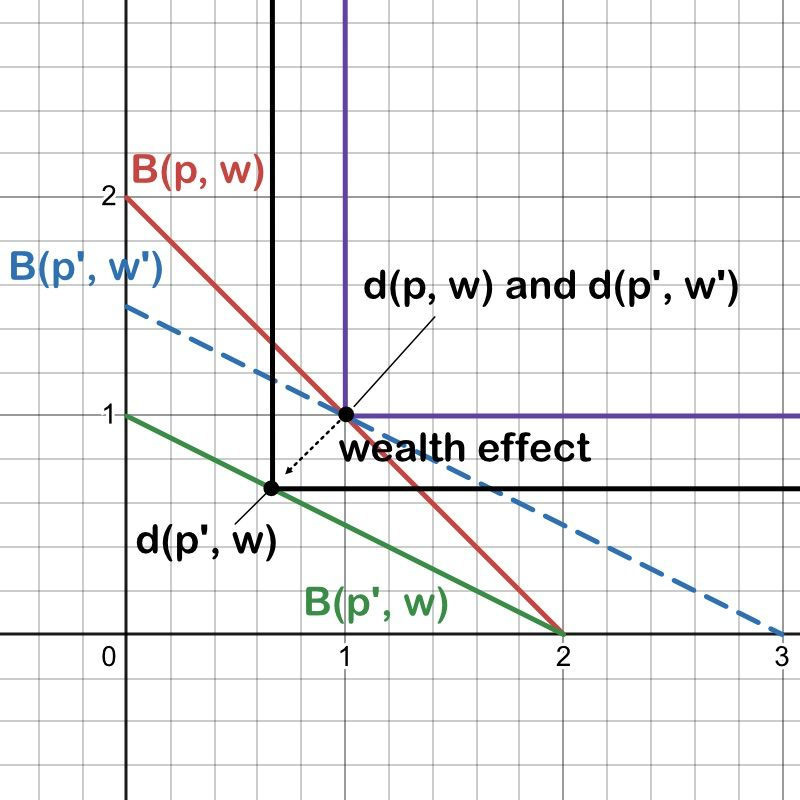
\includegraphics[width=0.5\linewidth]{assets/decision-theory/ps2-ex2.jpg}
\end{figure}


\section*{Problem 3}
\stepcounter{section}

We want to maximize the utility over the budget constraint.
To do so first we compute the Lagrangian
\begin{equation}
	\mathcal L(c_1, c_2, \lambda) = \frac{c_1 -1}{(2 - c_2)^2} + \lambda(w - p_1 c_1 - p_2 c_2)
\end{equation}
and its derivatives
\begin{equation}
	\begin{cases}
		\pdv{\mathcal L}{c_1} = \frac{1}{(2-c_2)^2} - \lambda p_1 \\
		\pdv{\mathcal L}{c_2} = \frac{2(c_1 - 1)}{(2-c_2)^3} - \lambda p_2
	\end{cases}
\end{equation}
now set them equal to $0$ and find $\lambda$
\begin{equation}
	\begin{cases}
		\lambda = \frac{1}{p_1 (2-c_2)^2} \\
		\lambda = \frac{2(c_1 - 1)}{p_2 (2-c_2)^3}
	\end{cases}
\end{equation}
therefore
\begin{equation}
	\frac{1}{p_1 (2-c_2)^2} = \frac{2(c_1 - 1)}{p_2 (2-c_2)^3}
	\implies c_1 = \frac{p_2(2-c_2)}{2p_1} + 1
\end{equation}

Now we can substitute this result back into the budget constraint giving us
\begin{equation}
	p_1 \left( \frac{p_2(2-c_2)}{2p_1} + 1 \right) + p_2 c_2 = w
	\implies c_2 = \frac{2(w - p_1 - p_2)}{p_2}
\end{equation}
and by substituting the value of $c_2$ back into $c_1$ we get the desired result:
\begin{equation}
	\begin{cases}
		d_1(w, p) = c_1 = 2 - \frac{w - 2p_2}{p_1} \\
		d_2(w, p) = c_2 = \frac{2(w - p_1)}{p_2} - 2
	\end{cases}
\end{equation}

\section*{Problem 4}
\stepcounter{section}

\subsection*{Part 1}
\begin{equation}
	E(l_1) = 4 \cdot 0.75 + 7 \cdot 0.25 = 4.75
\end{equation}
and
\begin{equation}
	E(l_2) = 3 \cdot 0.5 + 6 \cdot 0.25 + 7 \cdot 0.25 = 4.75
\end{equation}
so
\begin{equation}
	(E(l_1), 1) = (4.75, 1) \sim l_1
\end{equation}
and
\begin{equation}
	(E(l_2), 1) = (4.75, 1) \sim l_2
\end{equation}
by transitivity, we have
\begin{equation}
	l_1 \sim (4.75, 1) \sim l_2 \implies l_1 \sim l_2
\end{equation}
Thus, a risk-neutral decision maker can choose either lottery.

\subsection*{Part 2}
For individual $A$,
\begin{equation}
	l_1 \succsim l_2 \iff \sum_{i = 1}^n u_A({c_1}_i) p_i \ge \sum_{i = 1}^n u_A({c_2}_i) p_i
\end{equation}
Computing the inequality, we get
\begin{align}
	\sqrt{4} \cdot 0.75 + \sqrt7 \cdot 0.25 & \lesseqgtr \sqrt3 \cdot 0.5 + \sqrt6 \cdot 0.25 + \sqrt7 \cdot 0.25 \\
	2.16                                    & \ge 2.14                                                            \\
	l_1                                     & \succsim l_2
\end{align}
So individual $A$ would choose $l_1$. Since $u_A(c) = \sqrt c$ is concave, individual $A$ is risk-averse.

For individual $B$,
\begin{equation}
	l_1 \succsim l_2 \iff \sum_{i = 1}^n u_B({c_1}_i)p_i \ge \sum_{i = 1}^n u_B({c_2}_i) p_i
\end{equation}
Computing
\begin{align}
	4^2 \cdot 0.75 + 7^2 \cdot 0.25 & \lesseqgtr 3^2 \cdot 0.5 + 6^2 \cdot 0.25 + 7^2 \cdot 0.25 \\
	24.25                           & \le 25.75                                                  \\
	l_1                             & \precsim l_2
\end{align}
So individual $B$ would choose $l_2$. Since $u_B(c) = c^2$ is convex, individual $B$ is risk-loving.

\subsection*{Part 3}
Given the utility function $u_A(c) = \sqrt c$,
the certain equivalents for individual $A$ are the values computed in the previous part,
\begin{equation}
	c_{l_1} = \sqrt4 \cdot 0.75 + \sqrt7 \cdot 0.25 = 2.16
\end{equation}
and
\begin{equation}
	c_{l_2} = \sqrt3 \cdot 0.5 + \sqrt6 \cdot 0.25 + \sqrt7 \cdot 0.25 = 2.14
\end{equation}
The risk premiums are
\begin{equation}
	\pi_{l_1} = E(l_1) - c_{l_1} = 4.75 - 2.16 = 2.59
\end{equation}
and
\begin{equation}
	\pi_{l_2} = E(l_2) - c_{l_2} = 4.75 - 2.14 = 2.61
\end{equation}

Similarly, given the utility function $u_B(c) = c^2$, the certain equivalents for individual $B$ are
\begin{equation}
	c_{l_1} = 4^2 \cdot 0.75 + 7^2 \cdot 0.25 = 24.25
\end{equation}
and
\begin{equation}
	c_{l_2} = 3^2 \cdot 0.5 + 6^2 \cdot 0.25 + 7^2 \cdot 0.25 = 25.75
\end{equation}
The risk premiums are
\begin{equation}
	\pi_{l_1} = E(l_1) - c_{l_1} = 4.75 - 24.25 = -19.5
\end{equation}
and
\begin{equation}
	\pi_{l_2} = E(l_2) - c_{l_2} = 4.75 - 25.75 = -21
\end{equation}

\section*{Problem 5}
\stepcounter{section}

Let us write $u(c)$ as
\begin{equation}
	u(c) = \frac{1}{2} u(c + k) + \frac{1}{2} u(c-k) + \pi(c, k, u) [ u(c + k) - u(c-k)]
\end{equation}

Then, since $u$ is concave, by choosing $\alpha = \frac{1}{2}$ we get
\begin{equation}
	u(\alpha (c - k) + (1-\alpha) (c + k)) = u(c) \geq \alpha u(c - k) + (1-\alpha) u(c+k) = \frac{1}{2} u(c + k) + \frac{1}{2} u(c-k)
\end{equation}
which means that $\pi(c, k, u) [ u(c + k) - u(c-k)] \geq 0$.

Moreover, since $u$ is increasing, $u(c + k) - u(c-k) \geq 0$, hence, necessarily $\pi(c, k, u) \geq 0$ too.

\end{document}
